% !TeX root = ./Dyplom.tex

\chapter{Generowanie reprezentacji wektorowej wypowiedzi}
	Reprezentacje wektorowe słów (ang. word embedding)
\section{BERT}



  Podział na zdania - trza bo:
  \begin{figure}[ht]
    \begin{minipage}{.75\textwidth}\label{fig:word_count}
      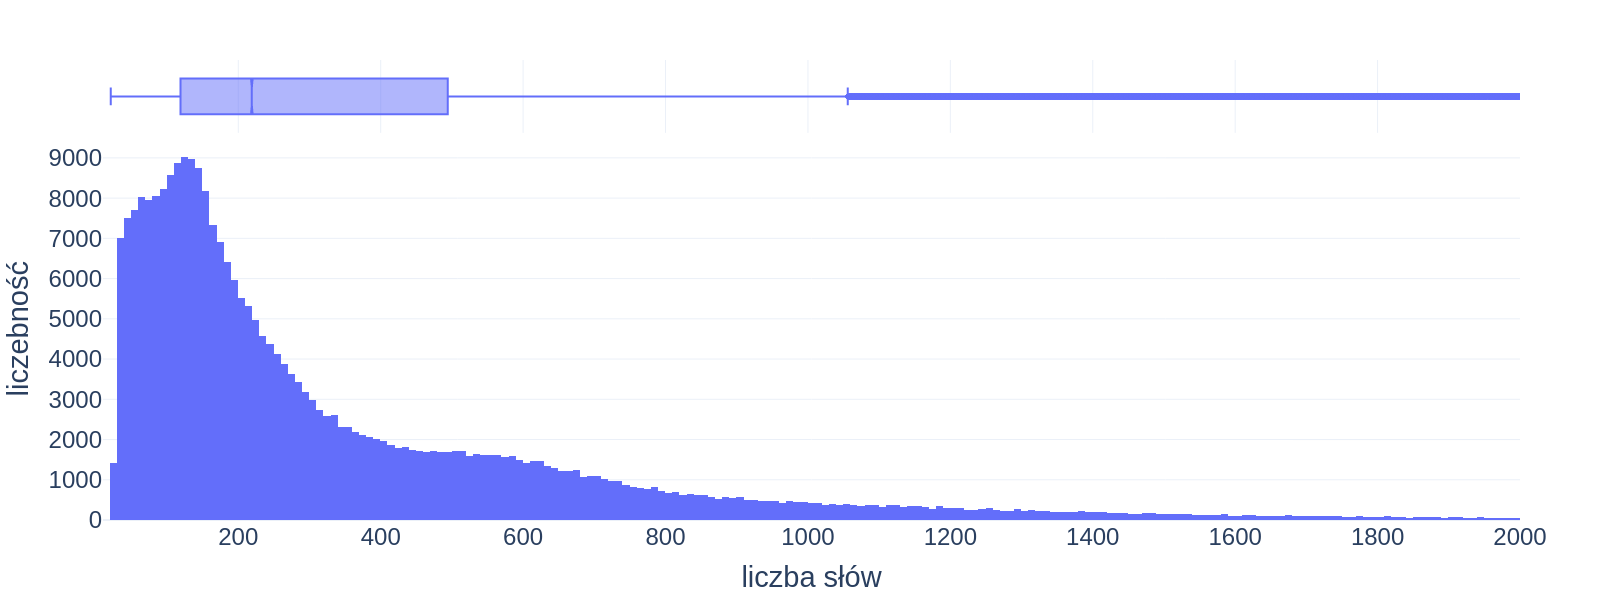
\includegraphics[width=\textwidth]{rys03/word_count.png}
    \end{minipage}%
    \begin{minipage}{.25\textwidth}\label{tab:word_count}
      \small
      \begin{tabularx}{\textwidth}{l|l}
        Min & 21 \\ 
        Q1 & 119 \\ 
        Mediana & 219 \\
        Q3 & 494 \\ 
        Górny wąs & 1056 \\
        Max & 28.546 \\
      \end{tabularx}
    \end{minipage}
    \caption{Dystrybucja długości wypowiedzi (zakres do 2000 słów)}
  \end{figure}